\documentclass[11pt]{article}
    \title{\textbf{Stat 265 Homework I}}
    \author{Khac Nguyen Nguyen}
    \date{}
    
    \addtolength{\topmargin}{-3cm}
    \addtolength{\textheight}{3cm}
    
\usepackage{amsmath}
\usepackage{mathtools}
\usepackage[dvipsnames]{xcolor}
\usepackage{tikz}
\begin{document}	



\section*{1.}
Let $B$ be the event where committees can be formed without any restriction and $C$ be the event where committes are formed with both Charlotte and Leonard.
\[
n_B = 
\begin{pmatrix}
6 \\
3
\end{pmatrix}
\cdot
\begin{pmatrix}
8 \\
5
\end{pmatrix}
\cdot
\begin{pmatrix}
3 \\
2
\end{pmatrix}
= 3360
\]
\[n_C =
\begin{pmatrix}
6 \\
3
\end{pmatrix}
\cdot
\underbrace{
\begin{pmatrix}
7 \\
4
\end{pmatrix}
}_{\substack{{\text{Charlotte}} \\ \text{is chosen}}}
\cdot
\underbrace{
\begin{pmatrix}
2 \\
1
\end{pmatrix}
}_{\substack{{\text{Leonard}} \\ \text{is chosen}}}
=1400
\]
\[
n_A = n_B - n_C = 1960
\]
\pagebreak
\section*{2.}
a.
Since A is the event where there is at least one ace chosen, $\overline{A}$ is the event where there is no aces chosen.
\[
n_{\overline{A}}= 
\begin{pmatrix}
48 \\
5
\end{pmatrix} 
= 1712304
\] where 48 is the number of non-ace card in the deck. Also
\[n=
\begin{pmatrix}
52 \\
5
\end{pmatrix}
= 2598960
\]
Therefore, the probability that there are no ace chosen is
\[
P(\overline{A}) = 
\frac{n_{\overline{A}}}{n} =
\frac{1712304}{2598960}
\]
and the probability that there is at least one ace chosen is 
\[
P(A) = 1 - p(\overline{A}) = \frac{886656}{2598960}
\]
b.
Since we are choosing 5 cards with different denominations, we are choosing 5 denominations from the 13 denominations. For each denominations, we can choose a suit out of 4 suits. Therefore,
\[n_D = 
\begin{pmatrix}
13 \\
5
\end{pmatrix}
\cdot
\begin{pmatrix}
4 \\
1
\end{pmatrix}^5= 1317888
\]
Hence, 
\[
P(D) = 
\frac{n_D}{n} =
\frac{1317888}{2598960}
\]
c.
The probability that a hand of 5 different denominations are dealt and 1 one of them is an ace is similar to part b with a minor change\\
\[
P(A\cap D) = 
\frac{n_{A \cap D}}{n} =
\frac{
\overbrace{
\begin{pmatrix}
12\\
4
\end{pmatrix}
}^{\substack{\text{Ace is} \\ \text{chosen}}
}
\cdot
\begin{pmatrix}
4 \\
1
\end{pmatrix}^5}
{\begin{pmatrix}
52 \\
5
\end{pmatrix}} 
= \frac{2112}{10829}
\]
We have 
\[
P(A\cup D)  = P(A)+P(D)-P(A\cap D) = \frac{35368}{54145}
\]
\pagebreak
\section*{3.}
The number of ways the deck can be dealt is 
\[
n =
\begin{pmatrix}
&9\\
3 & 3 & 3
\end{pmatrix}
= 1680
\]
Let $T_i$ be the event where player i is dealt three of a kind.

\[
n_{T_1 \cap T_2 \cap T_3} = 
\begin{pmatrix}
& 3 \\
1 & 1 & 1
\end{pmatrix}
= 6
\]
because there is 3 denominations and each player choose 1.
\[
n_{\overline{T}_1 \cap T_2 \cap T_3} = n_{T_1 \cap \overline{T}_2 \cap T_3} = n_{T_1 \cap T_2 \cap \overline{T}_3} = 0 
\]
because if 2 player are dealt three of a kind then the rest 3 cards are of the same denomination, which means it is impossible for the third player not being dealt three of a kind. \\~\\
The number of ways player 1 is dealt three of a kind is 
\[
n_{T_1} = 
\underbrace{
3 \cdot
\begin{pmatrix}
& 3 \\
3 & 0 & 0
\end{pmatrix}
}_{
\substack{
\text{There is 3 different} \\
\text{denominations player 1 can get }
}}
\cdot 
\underbrace{
\begin{pmatrix}
& 6 \\
0 & 3 & 3
\end{pmatrix}
}_{\text{Player 2 and 3}}
= 3 \cdot 1 \cdot 20 = 60
\]
\begin{equation*}
\begin{aligned}
n_{T_1 \cap \overline{T}_2 \cap \overline{T}_3} 
&= n_{T_1}-n_{T_1 \cap \overline{T}_2 \cap T_3} - n_{T_1 \cap T_2 \cap \overline{T}_3} - n_{T_1 \cap T_2 \cap T_3}\\
&= 60 - 0 - 0 - 6 = 54
\end{aligned}
\end{equation*}
WLOG,
\[n_{\overline{T}_1 \cap T_2 \cap \overline{T}_3} = n_{\overline{T}_1 \cap \overline{T}_2 \cap T_3} = 54\]
Therefore, the total number of ways one player is dealt three of a kind is
\begin{equation*}
\begin{aligned}
n_A &= n_{T_1 \cap \overline{T}_2 \cap \overline{T}_3}  + n_{\overline{T}_1 \cap T_2 \cap \overline{T}_3} + n_{\overline{T}_1 \cap \overline{T}_2 \cap T_3} \\ 
&+n_{\overline{T}_1 \cap T_2 \cap T_3} + n_{T_1 \cap \overline{T}_2 \cap T_3} + n_{T_1 \cap T_2 \cap \overline{T}_3} \\
&+ n_{T_1 \cap T_2 \cap T_3} \\
&= 54+54+54+0+0+0+6 = 168
\end{aligned}
\end{equation*} 
Hence the probability is
\[
P(A) = \frac{168}{1680} = \frac{1}{10}
\]
\pagebreak
\section*{4.}
Let A, B respectively be the event where the product is manufacture from machine A and B. \\
Let D be the event where the product is defective. 
We have
\[P(B|D) = 0.65 \implies P(A|D) = 1-0.65 = 0.35\]
and
\[P(D|A) = 3 \cdot P(D|B)\]
\begin{equation*}
\begin{aligned}
&\implies P(A|D) \cdot \frac{P(D)}{P(A)}= 3 \cdot P(B|D) \cdot \frac{P(D)}{P(B)} \\
&\implies 0.35 \cdot \frac{1}{P(A)} = 3 \cdot 0.65 \cdot \frac{1}{P(B)} \\
&\implies P(A) = \frac{7}{39} P(B)
\end{aligned}
\end{equation*}
We also have 
\[P(A) + P(B) = 1\]
\begin{equation*}
\begin{aligned}
& \implies  \frac{7}{39} P(B) + P(B) = 1 \\
& \implies P(B) = \frac{39}{46} = 84.783\%
\end{aligned}
\end{equation*}



\pagebreak
\section*{5.}
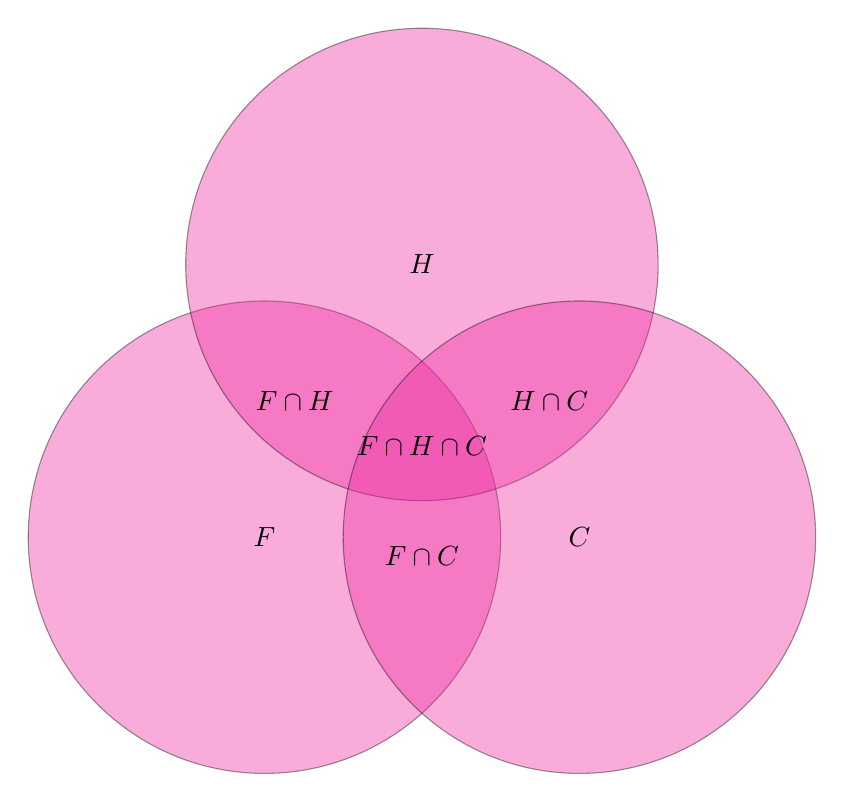
\begin{tikzpicture} [set/.style = {draw,
    circle,
    minimum size = 6cm,
    fill=Rhodamine,
    opacity = 0.4,
    text opacity = 1}]
 
\node (F) [set] {$F$};
\node (H) at (60:4cm) [set] {$H$};
\node (C) at (0:4cm) [set] {$C$};
 
\node at (barycentric cs:F=1,H=1) [left] {$F\cap H$};
\node at (barycentric cs:F=1,C=1) [below] {$F \cap C$};
\node at (barycentric cs:H=1,C=1) [right] {$H \cap C$};
\node at (barycentric cs:F=1,H=1,C=1) [] {$F \cap H \cap C$};
 
\end{tikzpicture}
\\
We know that $P(F) = 0.25,P(H)= 0.4, P(C)=0.3, P(F \cap H) = 0.15, P(H \cap C) = 0.2, P(F \cap C) = 0.1, P(F \cap H \cap C) = 0.05$ \\
From the diagram, we can see that \\
$P(F\cap \overline{H} \cap C) = P(F\cap C) - P(F \cap C \cap H) =  0.1 - 0.05 = 0.05$ \\
$P(\overline{F}\cap H \cap C) = P(H\cap C) - P(F \cap C \cap H) =  0.2 - 0.05 = 0.15$ \\
$P(F\cap H \cap \overline{C}) = P(F\cap H) - P(F \cap C \cap H) =  0.15 - 0.05 = 0.1$ \\
\begin{equation*}
\begin{aligned}
P(F \cap \overline{H} \cap \overline{C}) &= P(F) - P(F\cap H \cap \overline{C}) - P(F\cap \overline{H} \cap C)  - P(F\cap H \cap C) \\
&= 0.25 - 0.1 - 0.05 - 0.05 = 0.05
\end{aligned}
\end{equation*}
\begin{equation*}
\begin{aligned}
P(\overline{F} \cap \overline{H} \cap C) &= P(C) - P(F\cap \overline{H} \cap C) - P(\overline{F} \cap H \cap C)  - P(F\cap H \cap C) \\
&= 0.3-0.05 - 0.15 -0.05 = 0.05
\end{aligned}
\end{equation*}
\begin{equation*}
\begin{aligned}
P(\overline{F} \cap H \cap \overline{C}) &= P(H) - P(F\cap H \cap \overline{C}) - P(\overline{F} \cap H \cap C)  - P(F\cap H \cap C) \\
&= 0.4-0.1-0.15-0.05 = 0.1
\end{aligned}
\end{equation*}
Therefore, the proportion of individuals watch exactly one of the sports is $0.05+0.05+0.1=0.2=20\%$
\pagebreak
\section*{6.}
a. For the game to end at exactly 10-th turn, the winner has to win 8 times and loses 2 times, the the loser loses 8 times and win 2 times. Also, the loser must not go bankrupt before round 10 and the loser must lose the 10-th round. \\
First, we consider the first 6 rounds, if the winner win all 6 round, the loser goes bankrupt which means the game ends at the 6-th round, therefore, the loser must win at least 1 game, and at most 2 game. \\
If the loser win 1 game, then at the end of round 6, the loser has 2 dollars, and the loser must win on round 7 or 8 so that the game does not end because if the loser lose both round 7 and 8 he goes bankrupt at round 8. Hence, the number of ways the game ends at round 10 if the loser win 1 game in the first 6 round is 
\[
\begin{pmatrix}
6 \\ 
1
\end{pmatrix}
\cdot 
\begin{pmatrix}
2 \\ 
1
\end{pmatrix} = 12
\]
If the loser win 2 game before round 6, then the loser is safe to not go bankrupt before round 10. Hence the probability the game ends at round 10 if the loser win 2 games in the first 6 round is 
\[
\begin{pmatrix}
6 \\ 
2
\end{pmatrix}
= 15
\]
Therefore, the probability the game end in exactly 10 round is 
\[
2 \cdot
(15+12)
\cdot 
\left( \frac{1}{2} \right)^8
\cdot
\left( \frac{1}{2} \right)^2
= \frac{54}{1024}
\]
as any player can be the winner. \\
b. Consider a one player game where the player has i dollars where i is less than or equal to 5, each round, the player has a probability of p winning 1 dollar and if he does not win, the player loses 1 dollar. The player win the game when he reached 5 dollars and loses when he go bankrupt, that is he reached 0 dollar.
Let P(i) be the possibility that the player win the game when he starts with i dollars. \\
Then we have the following: 
\begin{equation*}
\begin{aligned}
&P(0) = 0, P(5) = 1 \\
&P(1) = (1-p)P(0) + pP(2) = pP(2) \\
&P(4) = pP(5) + (1-p)P(3) = p + (1-p)P(3)\\
&P(3) = (1-p)P(4) + pP(2) = (1-p)(p + (1-p)P(3)) + pP(2) \\
\implies &P(3) = P(2)(1-p) + p^2 + (p-p^2)P(3) \\
\implies &P(3)(1-p+p^2) = P(2)(1-p) + p^2 \\
\implies &P(3) = \cfrac{P(2)(1-p) + p^2}{1-p+p^2} \\
&P(2) = (1-p)P(1) + pP(3) = (1-p)pP(2) + p \cdot \cfrac{P(2)(1-p) + p^2}{p^2-p+1} \\
\implies &P(2)\left(  1-p+p^2 + \cfrac{p^2-p}{p^2-p+1}\right) = \cfrac{p^3}{p^2-p+1} \\
\implies &P(2)\left(\cfrac{(p^2-p+1)^2 + p^2-p}{p^2-p+1}\right) = \cfrac{p^3}{p^2-p+1} \\
\implies &P(2) = \cfrac{p^3}{(p^2-p+1)^2 + p^2-p} \\
\implies &P(2) = \cfrac{p^3}{p^4-2p^3+4p^2-3p+1}
\end{aligned}
\end{equation*}
P(2) is the possibility that the player starts from 2 and then reaches 5 dollars without going bankrupt, which means that the possibility player A reaches 5 dollars without going bankrupt is the same, and since when player A reaches 5 dollars, player B has 0 dollar and go bankrupt. The possibility player A wins the game is similar to P(2) 
\pagebreak
\section*{7.}
Let $D_i$ be the event where i is rolled and $Q$ be the event where both the applicants are qualified
\[
P(D_4 \cup D_5 \cup D_6) = \frac{3}{6} = \frac{1}{2} 
\]
\[
P(Q | D_4 \cup D_5 \cup D_6) = \frac{8}{11} \cdot \frac{7}{11} = \frac{56}{121}
\]
\[
P(D_1 \cup D_2) = \frac{2}{6} = \frac{1}{3}
\]
\[
P(Q | D_1 \cup D_2) = \frac{8}{11} \cdot \frac{7}{10} = \frac{28}{55}
\]
\[
P(D_3) = \frac{1}{6}
\]
\[
P(Q | D_3) = \frac{7}{11} \cdot \frac{6}{10} = \frac{21}{55}
\]
\begin{equation*}
\begin{aligned}
P(Q) &= P(Q \cap (D_1 \cup D_2)) + P(Q \cap D_3) + P(Q \cap (D_4 \cup D_5 \cup D_6)) \\
& = P(Q | D_1 \cup D_2)P(D_1 \cup D_2) + P(Q | D_1 \cup D_3)P(D_3) \\
&+ (Q | D_4 \cup D_5 \cup D_6)P(D_4 \cup D_5 \cup D_6) \\ 
&= \frac{1}{2} \cdot \frac{56}{121} + \frac{1}{6} \cdot \frac{21}{55} + \frac{1}{3} \cdot \frac{28}{55} \\
&= \frac{1687}{3630}
\end{aligned}
\end{equation*}
\begin{equation*}
\begin{aligned}
P(D_4 \cup D_5 \cup D_6 | Q) &= \cfrac{P(D_4 \cup D_5 \cup D_6)}{P(Q)} \cdot P(Q | D_4 \cup D_5 \cup D_6) \\
&= \cfrac{\cfrac{1}{2}}{\cfrac{1687}{3630}} \cdot \cfrac{56}{121} = \cfrac{120}{241}
\end{aligned}
\end{equation*}
\pagebreak
\section*{8.}
Let $F_i$ be the event where the product is defective by factor $i$ and $T_i$ be the event where the test for the $i$ factor is positive.
We have \\ 
$P(F_1) = \cfrac{1}{36}, P(F_2) = \cfrac{8}{36}, P(F_3) = \cfrac{27}{36}$ \\
$P(T_1|F_1) = \cfrac{1}{5}, P(T_2|F_2) = \cfrac{2}{5}, P(T_3|F_3) = \cfrac{3}{5} $\\
$P(\overline{T}_m | F_n) = 
\begin{cases}
1 \text{ if } m\ne n \\
\cfrac{5-m}{5} \text{ otherwise}
\end{cases} 
$

a. 
\begin{equation*}
\begin{aligned}
P(\overline{T}_1) &= P(\overline{T}_1 \cap F_1) + P(\overline{T}_1 \cap F_2)  +P(\overline{T}_1 \cap F_3) \\
&= P(\overline{T}_1 | F_1)P(F_1) + P(\overline{T}_1 | F_2)P(F_2)  +P(\overline{T}_1 | F_3)P(F_3) \\
&= \cfrac{4}{5} \cdot \cfrac{1}{36} + 1 \cdot \cfrac{8}{36} + 1 \cdot  \cfrac{27}{36} = \cfrac{179}{180}\\
P(F_1|\overline{T}_1) &= P(\overline{T}_1 | F_1) \cdot \cfrac{P(F_1)}{P(\overline{T}_1)} \\
&= \cfrac{4}{5} \cdot \frac{\cfrac{1}{36}}{\cfrac{179}{180}} = \cfrac{4}{179} 
\end{aligned}
\end{equation*}
b.
\begin{equation*}
\begin{aligned}
P(\overline{T}_2) &= P(\overline{T}_2 \cap F_1) + P(\overline{T}_2 \cap F_2)  +P(\overline{T}_2 \cap F_3) \\
&= P(\overline{T}_2 | F_1)P(F_1) + P(\overline{T}_2 | F_2)P(F_2)  +P(\overline{T}_2 | F_3)P(F_3) \\
&= 1 \cdot \cfrac{1}{36} + \cfrac{3}{5}  \cdot \cfrac{8}{36} + 1 \cdot  \cfrac{27}{36} = \cfrac{41}{45}\\
P(F_3|\overline{T}_2) &= P(\overline{T}_2 | F_3) \cdot \cfrac{P(F_3)}{P(\overline{T}_2)} \\
&= 1 \cdot \frac{\cfrac{27}{36}}{\cfrac{41}{45}} = \cfrac{135}{164} 
\end{aligned}
\end{equation*} 
\pagebreak
\section*{9.}
In case Bert goes first, Bert can only win on odd turns, which means that he can only win on 2k+1 turn where k $\ge$ 0.
The possibility Bert wins on the 2k+1 turn is 
\[\underbrace{(0.8)^k (0.7)^k}_{\substack{\text{each player} \\ \text{lose k turns}}}\underbrace{(0.2)}_{\substack{\text{Bert wins} \\ \text{the last turn}}} = (0.56)^k(0.2)\]
Therefore, the possibility Bert wins if Bert goes first is 
\[
\sum_{k=0}^\infty (0.56)^k(0.2) = \cfrac{0.2}{1-0.56} = \cfrac{5}{11}
\]
In case Earnie goes first, Bert can only win on even turns, which means that he can only on 2k+2 turn where k $\ge$ 0. The possibility Bert wins on the 2k+2 turn is
\[
\underbrace{(0.8)^k (0.7)^k}_{\substack{\text{each player} \\ \text{lose k turns}}}
\underbrace{(0.7)}_{\substack{\text{Earnie losess the} \\ \text{2nd last turn}}}
\underbrace{(0.2)}_{\substack{\text{Bert wins} \\ \text{the last turn}}} = (0.56)^k(0.14)
\]
Therefore, the possibility Bert wins if Earnie goes first is 
\[
\sum_{k=0}^\infty (0.56)^k(0.14) = \cfrac{0.14}{1-0.56} = \cfrac{7}{22}
\]
Since the coin is fair, the possibility that Bert goes first is 0.5 and the possibility that Earnie goes first is 0.5, hence the possibility that Bert wins is 
\[
\cfrac{1}{2} \cdot \cfrac{5}{11} + \cfrac{1}{2} \cdot \cfrac{7}{22} = \cfrac{17}{44}
\]
\pagebreak
\section*{10.}
a. Without replacement, player A gets 1 straws, player B gets 2 straws and player C gets 2 straws in the end. Therefore,
\[P(A)=\frac{1}{5}\]
\[P(B)=\frac{2}{5}\]
\[P(C)=\frac{2}{5}\]
b. With replacement, the probability player A must go on the mission at turn 5$k$+1 for $k\ge 0$ is
\[\left(\frac{1}{5}\right) {\left(\frac{4}{5}\right)}^{5k}\]
Hence, the probability player A win is 
\[P(A) = \left( \frac{1}{5} \right) \sum_{k=0}^{\infty} {\left( \frac{4}{5} \right)}^{5k}=\cfrac{625}{2101}\]
Similarly, the probability player B and C win are
\[P(B) = \left( \frac{1}{5} \right) \left( \frac{4}{5} \right) \sum_{k=0}^{\infty} {\left( \frac{4}{5} \right)}^{5k} + \left( \frac{1}{5} \right) {\left( \frac{4}{5} \right)}^4 \sum_{k=0}^{\infty} {\left( \frac{4}{5} \right)}^{5k} = \cfrac{500}{2101} + \cfrac{256}{2101} = \cfrac{756}{2101}\]
\[P(C) = \left( \frac{1}{5} \right) {\left( \frac{4}{5} \right)}^2 \sum_{k=0}^{\infty} {\left( \frac{4}{5} \right)}^{5k} + \left( \frac{1}{5} \right) {\left( \frac{4}{5} \right)}^3 \sum_{k=0}^{\infty} {\left( \frac{4}{5} \right)}^{5k} = \cfrac{400}{2101} + \cfrac{320}{2101} = \cfrac{720}{2101}\]
\end{document}


